% \newpage
\section{Hunting and Diffusion}
In this problem, we consider a population diffusion model which incorporates hunting. Firstly, we study the population size and stability in the presence of a hunting agent. Secondly, we analyze the same problem by incorporating spatial diffusion of the population. Finally, we also look at some scenarios where the terrain is non-uniform, resulting in a non-uniform population distribution and analyse the solution at different timestamps.

\subsection{Modelling population size}
Let $u$ be a function modelling a mobile population living in an environment with a growth rate of $r$\% per year with a carrying capacity of $K$. The typical equation that governs the size of the population is,

\begin{align}
    \frac{du}{dt} = ru \left(1 - \frac{u}{K}\right)
\end{align}

Now assume that hunters harvest $h$\% of the population per year. The above equation can account for this by adding an additional hunting term.

\begin{align} \label{hunting}
    \frac{du}{dt} = ru \left(1 - \frac{u}{K}\right) - hu
\end{align}

Eq. \ref{hunting} is a first-order nonlinear ordinary differential equation. The parameter space for $u$ can defined from $u\in [0, \infty)$, where the carrying capacity, $K \in \mathbb{R}^+$. We will see that after solving the differential equation the $u$ actually only goes from $0$ to $K$. Both $r, u \in [0,1]$, as they represent the fraction of population growing/getting hunted. Since this is an initial value problem, we need to provide some population size at time $t=0$. Assuming we need at least 2 organisms to reproduce, we provide $u(0)=2$. However the solution will not be much different with any other small value of $u(0)$.

We will now discuss how to numerically solve this differential equation. Note that the units of $r$ and $h$ throughout this section is [Time]$^{-1}$ and $u$ and $K$ are unitless. For simplicity, we won't be explicitly mentioning these units moving forward.

\subsubsection{Theoretical Approach}
The simplest method to solve a differential equation of the form $u' = f(u, t)$ is Euler's method. Here, we discretize time into steps of $\Delta t$. Given some initial conditions $u_i$, we approximate the next iteration as,

\begin{align}
    u_{i+1} = u_i + f(u_i, t_i)\Delta t
\end{align}

However, with large enough time steps, the error (of $O(h^2)$ in this case) accumulates, and the system quickly deviates from the actual solution. The implicit Euler's method however, tries to stabilize the solution by using

\begin{align}
    u_{i+1} = u_i + f(u_{i+1}, t_{i+1})\Delta t
\end{align}

However, while this is more numerically stable, this method undershoots the solution. For example, if we were solving this for a harmonic oscillator problem, the implicit Euler's method would appear to 'leak' energy. 

The Runge-Kutta method tries to fix the problem by taking a middle ground between the explicit and implicit Euler's methods to somewhat cancel out the deviations. Mathematically, the Runge-Kutta second order (RK2) method takes $k_1$ and $k_2$ as follows, as takes an average of the two values to calculate $u_{i+1}$.

\begin{align}
k_1 = f(u_i, t_i), k_2 &= f(u_i + k_1, t_i + \Delta t)\\
u_{i+1} &= u_i + \frac{dt}{2} (k_1+k_2)
\end{align}

Notice that the value we plug into $k_2$ is the same value we calculate for explicit Euler's method. Hence, here, the slope of the function at both increments is taken into account to calculate $u_{i+1}$.

This algorithm can be further improved by taking two extra weights to obtain the RK4 method. Here, we also consider the point $t_i + \Delta t/2$ and take the weighted average of four different slope values.

\begin{align}
    k_1 &= f(u_i, t_i) \nonumber\\
    k_2 &= f\left(u_i + k_1\frac{\Delta t}{2}, t_i+\frac{\Delta t}{2}\right) \nonumber\\
    k_3 &= f\left(u_i + k_2\frac{\Delta t}{2}, t_i+\frac{\Delta t}{2}\right) \nonumber\\
    k_4 &= f\left(u_i + k_3\Delta t, t_i+\Delta t\right) \nonumber\\
    u_{i+1} &= \frac{\Delta t}{6}(k_1+2k_2+2k_3+k_4)\nonumber\\
\end{align}

Where the weights for each $k$ value come from the Taylor series derivation.
RK4 is good enough for our purposes with a total accumulated error of the order $O(h^5)$.

\subsubsection{Results}
In Fig. \ref{5comps}, we have implemented forward Euler, Runge-Kutta 2 and Runge-Kutta 4 methods for a specific case where $r=0.5, h=0.25$, $K=100$ and $u(0)=2$. The real solution with these parameters was obtained analytically\footnote{\href{https://www.wolframalpha.com/input?i=y\%27+\%3D+0.5y*\%281-\%28y\%2F100\%29\%29-0.25y\%2C+y\%280\%29\%3D2}{Source.}} as $u(t) = \frac{50e^{t/4}}{24+e^{t/4}}$, which is also plotted in the figure.

\begin{figure}[H]
    \centering
    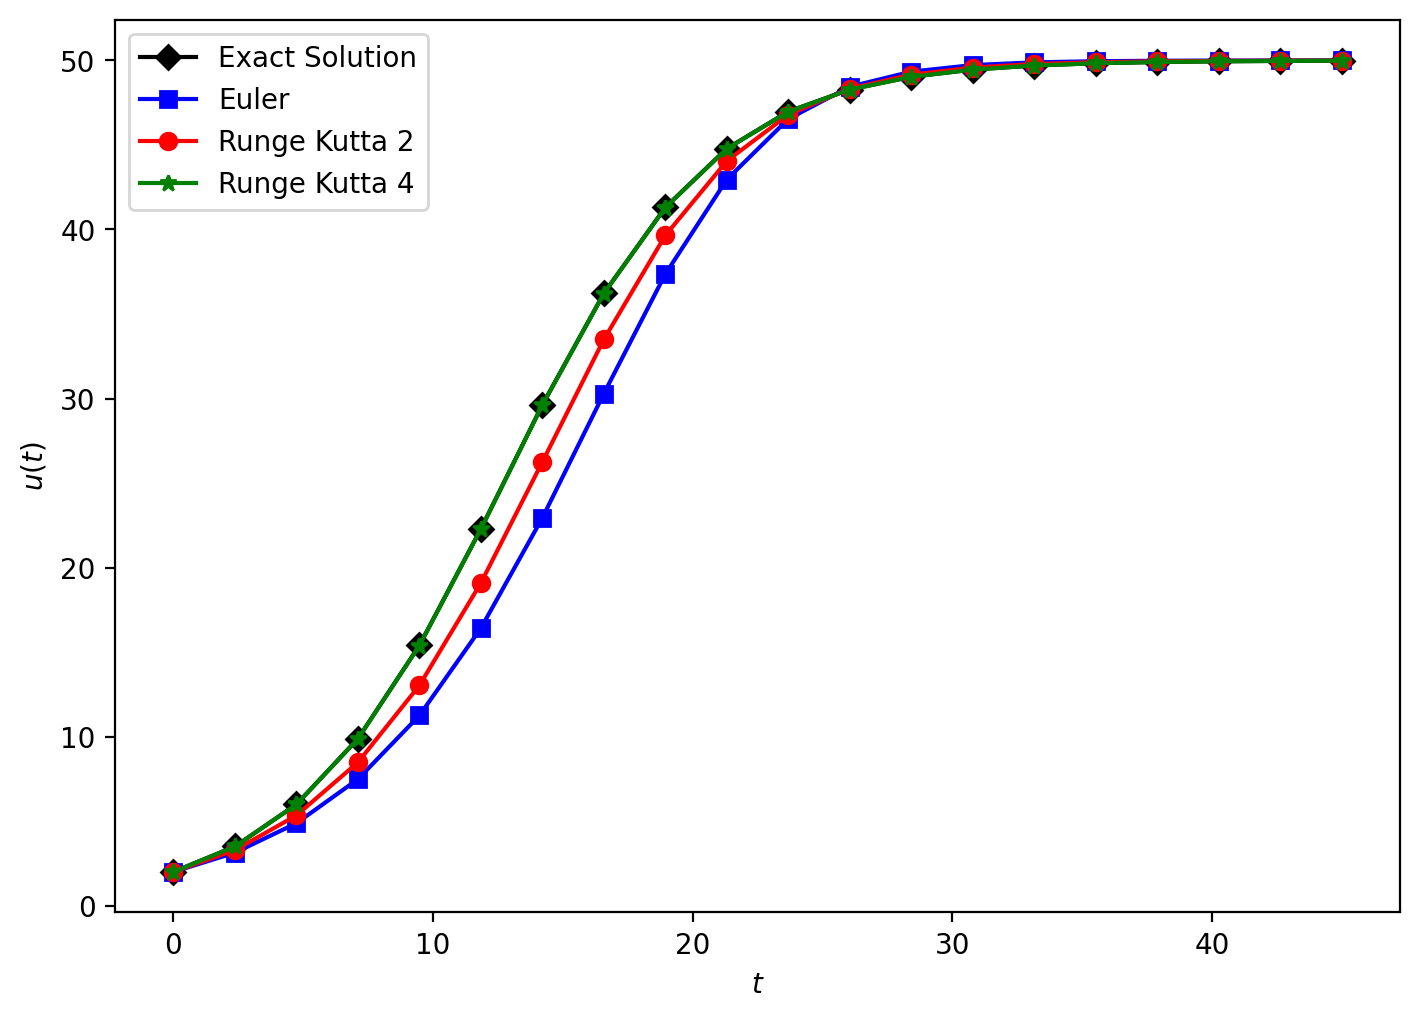
\includegraphics[width=0.6\linewidth]{Figures/5/5a/methods.png}
    \caption{Comparison of solutions obtained using 3 different methods compared with the real solution, with the same step sizes. Here, we can see that the RK4 method almost entirely overlaps the real solution, and RK2 is the second most accurate solution.}
    \label{5comps}
\end{figure}

In every case, we can see that the population size saturates after a certain amount of time at a much lower carrying capacity due to hunting. Solutions obtained using RK4 method for some other variations of parameters are shown below.

\begin{figure}[H]
     \centering
     \begin{subfigure}[b]{0.45\textwidth}
         \centering
         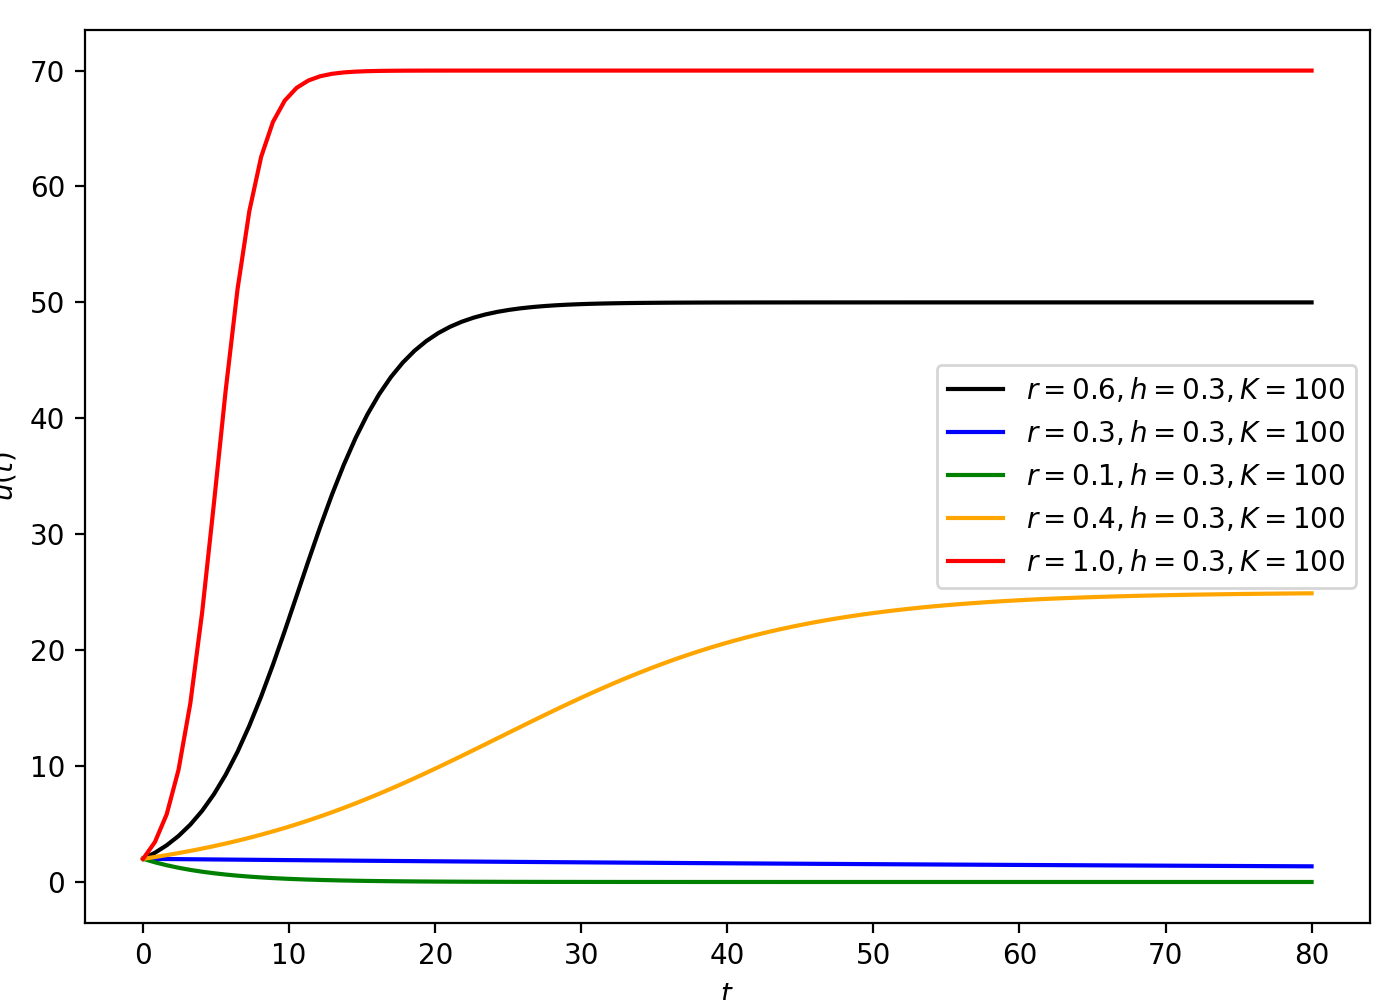
\includegraphics[width=\textwidth]{Figures/5/5a/varyR.png}
         \caption{With $h$ and $K$ kept constant, the time for saturation decreases and the saturated population increases with an increase in growth rate.}
     \end{subfigure}
     \begin{subfigure}[b]{0.45\textwidth}
         \centering
         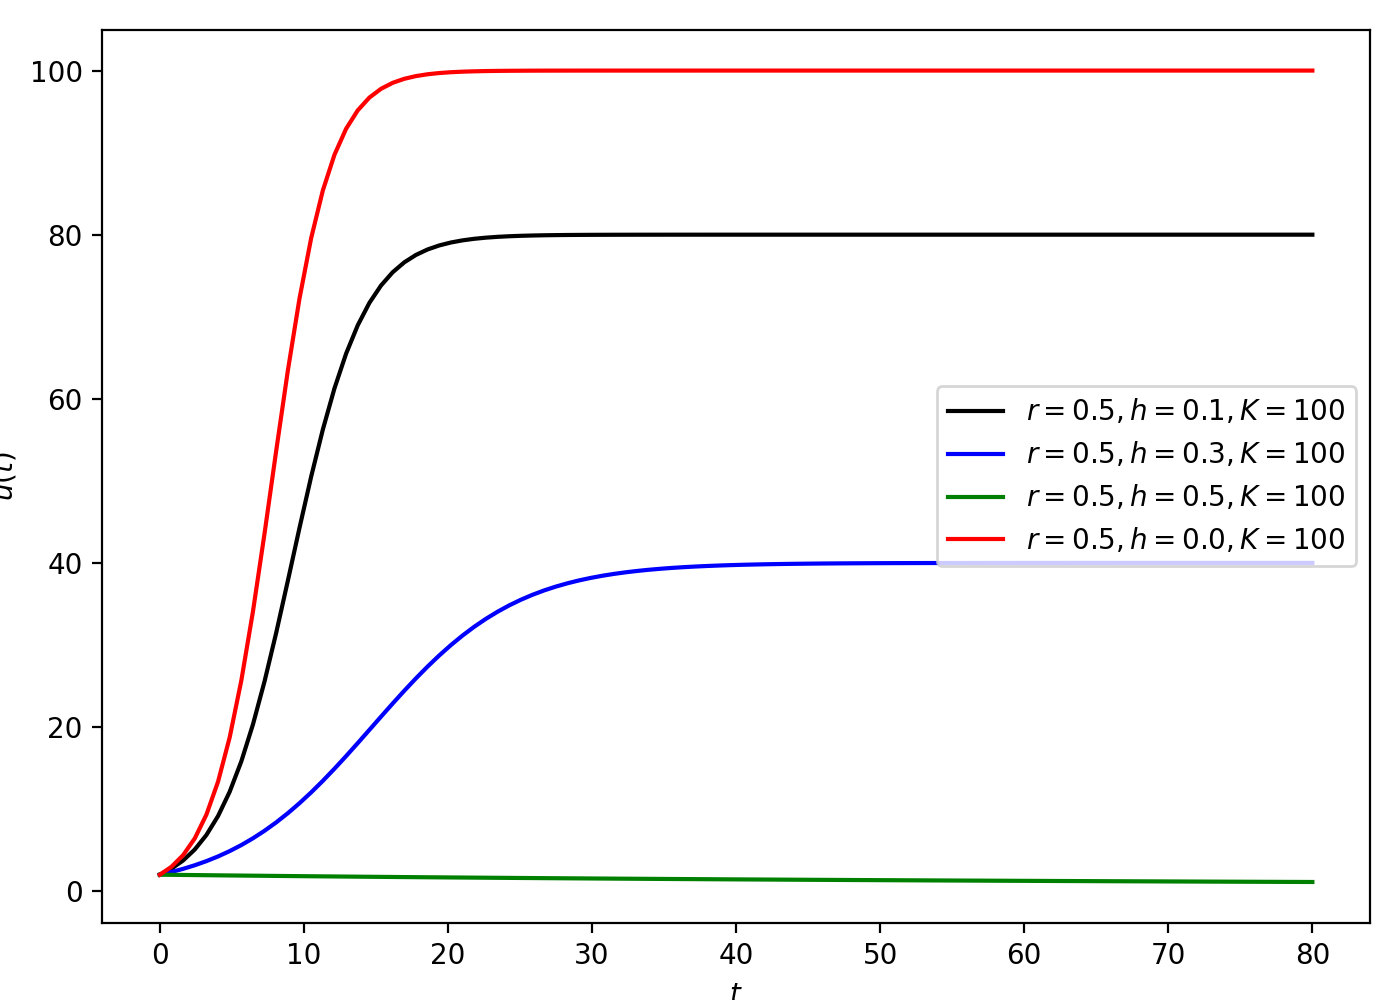
\includegraphics[width=\textwidth]{Figures/5/5a/varyH.png}
         \caption{With $r$ and $K$ kept constant, the population at saturation decreases with an increase in hunting rate as expected. When $h=0$, the population saturates at its carrying capacity.}
     \end{subfigure}
     \begin{subfigure}[b]{0.45\textwidth}
         \centering
         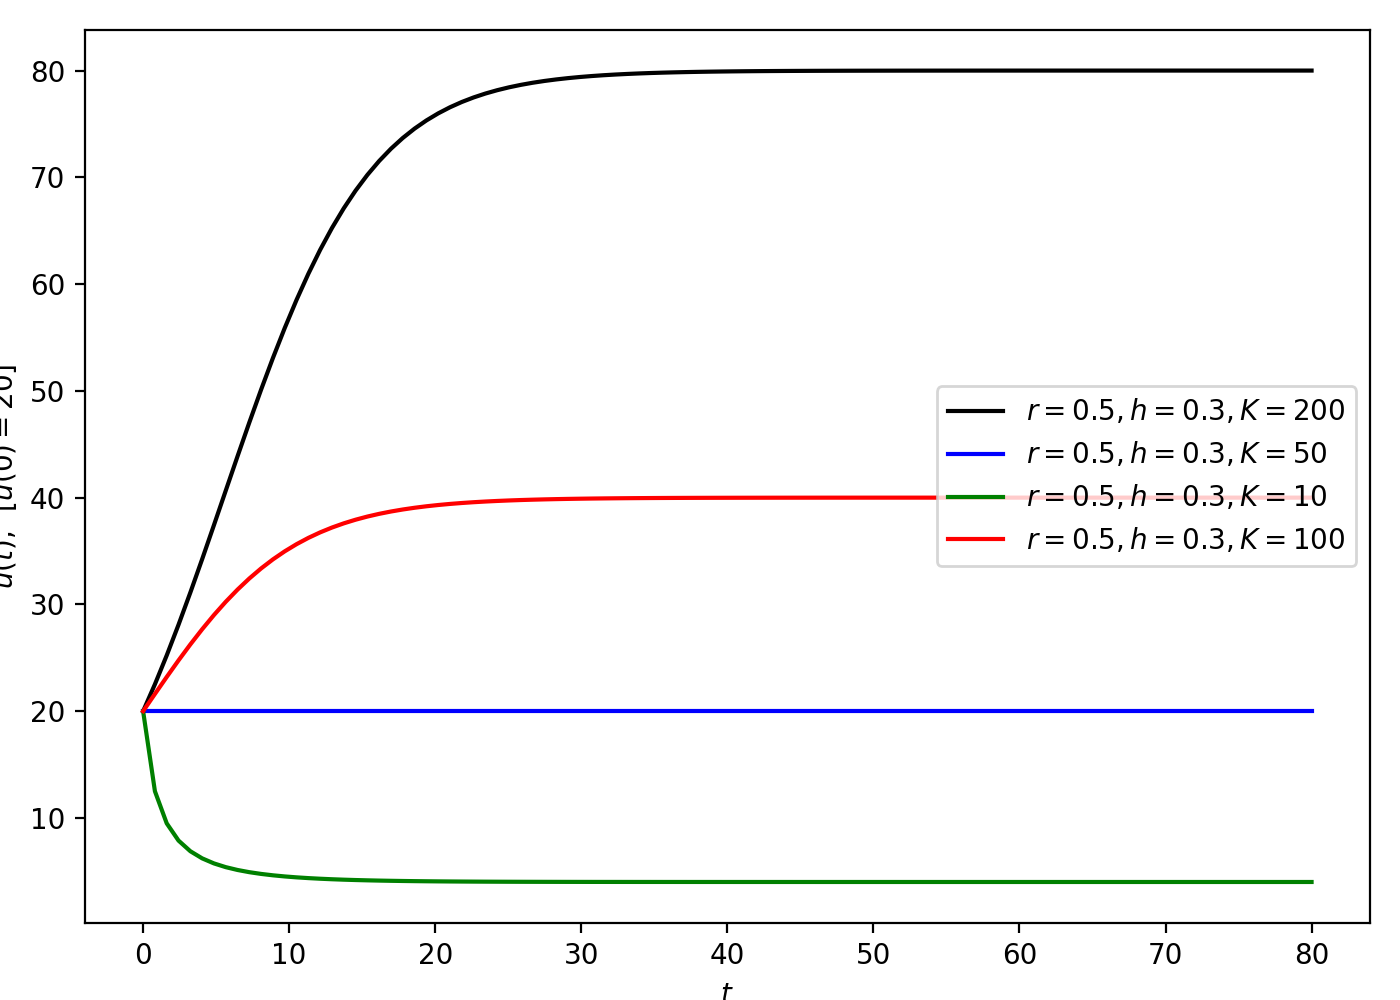
\includegraphics[width=\textwidth]{Figures/5/5a/varyK.png}
         \caption{With $r$ and $h$ kept constant, the population size at saturation varies proportionately with $K$. If $K<u(0)$, the population dies off eventually.}
     \end{subfigure}

    \caption{Solutions obtained for Eq. \ref{hunting} by systematically varying its parameters.}
\end{figure}

\subsection{Modelling the spread of individuals in a population}
Now, we want to model the spread of the mobile population. Before setting up the simulation, we will have 3 basic assumptions --

\begin{enumerate}
    \item Food is abundant in the entire environment.
    \item  Individuals in the population like to spread out so that they don’t interfere with each others’ hunt for food.
    \item It is equally easy for the individuals to travel in any direction in the environment.
\end{enumerate}

We can model the diffusion of the species through the environment by adding a diffusion term to Eq. \ref{hunting} and converting it into a partial differential equation, where $u$ is a function of $t, x$ and $y$. 

\begin{align} \label{diff+h}
    \frac{\partial u}{\partial t} = ru\left(1-\frac{u}{K}\right) - hu + D\left(\frac{\partial^2 u}{\partial x^2} + \frac{\partial^2 u}{\partial y^2}\right)
\end{align}

Here, $D > 0$ is the diffusion coefficient, indicating the ease of diffusion. To simplify the process we consider the 2D domain $(x, y) \in [0,1] \times [0,1]$ for the spatial part of this equation. Here, $K$ specifies the carry capacity per unit area.

Eq. \ref{diff+h} can be solved using methods described in section \ref{houses}. Here, we will be using the forward (or explicit) Euler method to calculate first and second derivatives. Since we are performing the calculation for every point in the grid, it will be much less computationally expensive than using higher order methods.

\subsubsection{Theoretical Approach}
We can implement Eq. \ref{diff+h} by discretising space and time into $\Delta x$ and $\Delta t$. Here we keep $\Delta x = \Delta y$ for simplicity. The equation can thus be rewritten as,

\begin{align}
    \frac{u_{i,j}^{(t+1)} - u_{i,j}^{(t)}}{\Delta t}  &= ru_{i,j}^{(t)} \left(1 - \frac{u_{i,j}^{(t)}}{K} \right) - hu_{i,j}^{(t)} + D \left( \frac{u_{i+1,j}^{(t)} -2u_{i,j}^{(t)} + u_{i-1,j}^{(t)}}{\Delta x^2} + \frac{u_{i,j+1}^{(t)} -2u_{i,j}^{(t)} + u_{i,j-1}^{(t)}}{\Delta y^2}\right)
\end{align}

Where $i,j$ represents the spatial coordinates for $t^\text{th}$ time snapsot. Here, we have used the finite difference approximation for second derivative to calculate the spatial diffusion part.

\begin{align}
    \frac{d^2f}{dx^2} = \frac{f(x+1) -2f(x) + f(x-1)}{\Delta x^2}
\end{align}

Now, we can rearrange to get $u_{i,j}^{(t+1)}$ as,

\begin{align}
    u_{i,j}^{(t+1)} = u_{i,j}^{(t)} + \Delta t\left[(r-h)u_{i,j}^{(t)} - \frac{r(u_{i,j}^{(t)})^2}{K} + \frac{D}{\Delta x^2} \left( u_{i+1,j}^{(t)} + u_{i-1,j}^{(t)} +  u_{i,j+1}^{(t)} + u_{i,j-1}^{(t)}  -4u_{i,j}^{(t)} \right)\right]
\end{align}

To implement boundary conditions for the spatial coordinates, we can add the Dirichlet boundary condition, $u|_{x,y=0}=0$. However, one can argue that the physical interpretation of the Dirichlet boundary condition, i.e. that the population dies off near the physical constraints of the boundary, does not make much sense. Hence, here we will apply the Neumann boundary condition, $\frac{\partial u}{\partial n}\big| _{x,y=0} = 0$. This makes sure that the population can spread evenly, even near the boundary points.

To implement Neumann boundary conditions, one can simply put

\begin{align}
    u_{i=0} = u_{i=1} \text{ and } u_{i=n} = u_{i=n-1}
\end{align}
for both $x$ and $y$ coordinates. This makes sure that their derivative at the boundary goes to zero.

\subsubsection{Implementation}

Here we have used the \verb|NUMBA| module which generates optimized machine code from pure Python to speed up the computation process.\\

\begin{lstlisting}[language=Python, caption=Code to simulate the hunting and diffusion model]
import numpy as np
import matplotlib.pyplot as plt
from matplotlib import animation
from mpl_toolkits.mplot3d import Axes3D
from matplotlib.animation import PillowWriter
from matplotlib import cm
import numba
from numba import jit

# Initialise space grid with 50 random spawns
n = 100
i = 5 # to avoid spawing any population near the edge 
coords = np.array([(np.random.randint(i, n-i), np.random.randint(i, n-i)) for _ in range (50)])
init_population = np.zeros((n, n))
for x, y in coords:
    init_population[x,y] = 2 # arbitrary initial value

# diffusion constant
D = 0.01

# set the dimensions of the problem
x = 1
dx = 0.05
dt = 0.0001 # such that D*dt/dx**2 < 1/4

times = 252000 # number of iterations
times_snapshot = 3600 # total number of snapshots
f = int(times/times_snapshot)

population_frames = np.zeros([times_snapshot, 100, 100])
population_frames[0] = init_population
population_density = np.zeros(times) # keeps track of the average population density

# Solving the PDE
# Set up numba function
@numba.jit("(f8[:,:,:], f8, f8, f8)", nopython=True, nogil=True, fastmath = True, parallel=True)
def solve_pde(environment, K, r, h):
    cs = environment[0].copy() #current state
    length = len(cs[0])
    density = np.zeros(times)
    density[0] = np.average(cs) # average population density
    cf = 0 # current frame

    for t in range(1, times):
        ns = cs.copy() # new state

        # Since only iterate spatially from 1 to n-1
        # the algorithm by design is implementing Dirichlet BCs
        for i in range(1, length-1):
            for j in range(1, length-1):
                growth = dt*((r-h)*cs[j][i] - (r*cs[j][i]**2)/K)
                diffusion = D*dt/dx**2 * (cs[j+1][i] + cs[j-1][i] +\
                                                    cs[j][i+1] + cs[j][i-1] -\
                                                    4*cs[j][i])
                ns[j][i] = cs[j][i] + diffusion + growth

        # Implementing Neumann BCs
        ns[:,0] = ns[:,1] # left boundary
        ns[:,-1] = ns[:,-2] # right boundary
        ns[0,:] = ns[1,:] # top boundary
        ns[-1,:] = ns[-2,:] # bottom boundary
        
        density[t] = np.average(cs)
        cs = ns.copy()
        if t%f==0: # take snapshot
            cf = cf + 1
            environment[cf] = cs
            
    return environment, density

# Setting up the parameters
K, r, h = 1, 0.9, 0.2

# Get population snapshots and population size over time and plot
population_frames, population_sizes = solve_pde(population_frames, K, r, h)
plt.plot(np.linspace(0, times*dt, times), population_sizes)
plt.xlabel('Time (s)')
plt.ylabel('Total Population')
plt.show()

# generate an animation of the simulation over time
def animate(i):
    ax.clear()
    im = ax.contourf(population_frames[10*i], 100, levels=np.linspace(0,np.max(population_sizes),50))
    plt.title(f't = {10*i*f*dt:.2f} sec')
    ax.set_xticks([]) 
    ax.set_yticks([]) 
    return fig,

fig, ax = plt.subplots(figsize=(8,6))
fig.colorbar(im, ax=ax)
ani = animation.FuncAnimation(fig, animate,
                               frames=359, interval=50)
ani.save('simulation.gif', writer='pillow', fps=30)
\end{lstlisting}

\subsubsection{Results}

Here are a few snapshots obtained in the simulation. The full simulation animations can be found \href{https://gayatri-p.github.io/p346-computational-physics/hunting2.html}{here}. 
As expected from the previous section, the population (initially spawned at random points) diffuses slowly until it reaches saturation.

\begin{figure}[H]
    \centering
    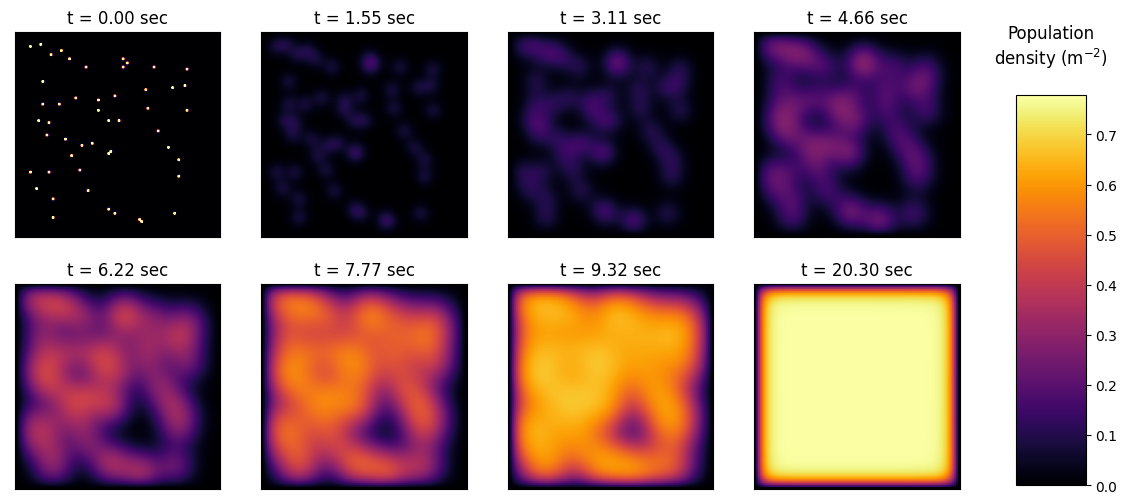
\includegraphics[width=1\linewidth]{Figures/5/5b/dirchlet.png}
    \caption{Snapshots of the environment at different times with Dirichlet Boundary Conditions ($r=0.9,h=0.2$)}
\end{figure}

\begin{figure}[H]
    \centering
    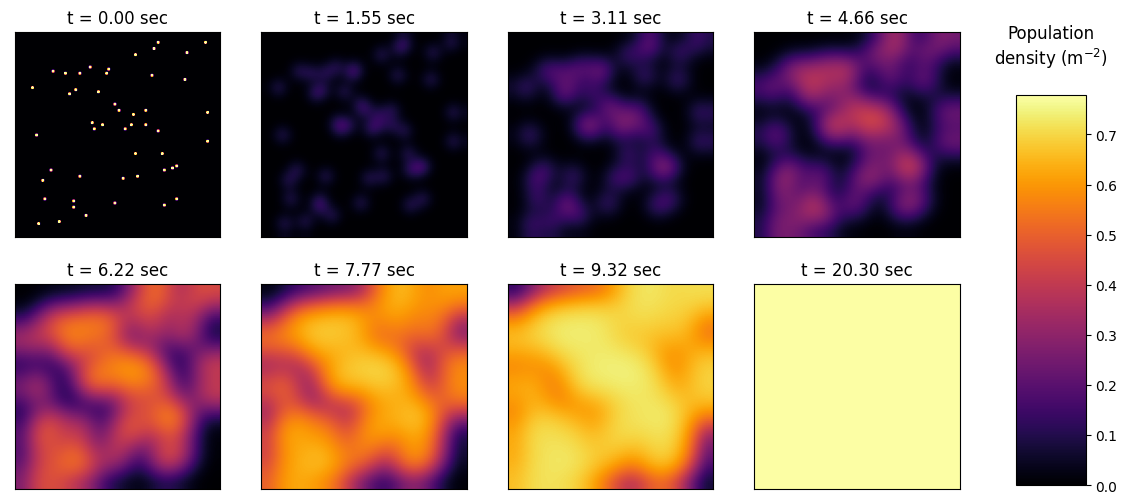
\includegraphics[width=1\linewidth]{Figures/5/5b/neumann.png}
    \caption{Snapshots of the environment at different times with Neumann Boundary Conditions ($r=0.9,h=0.2$)}
\end{figure}

\begin{figure}[H]
    \centering
    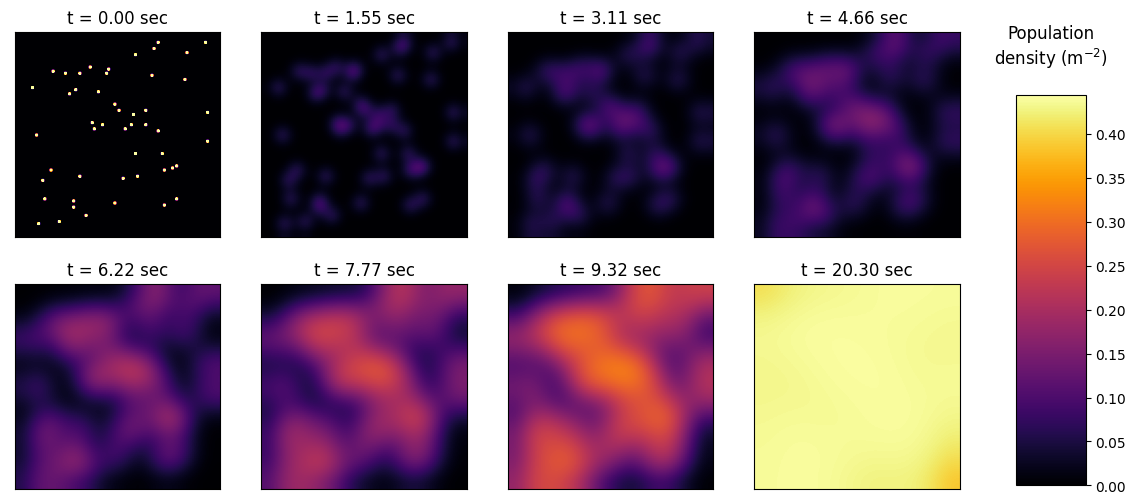
\includegraphics[width=1\linewidth]{Figures/5/5b/neumann_h5.png}
    \caption{Snapshots of the environment at different times with Neumann Boundary Conditions ($r=0.9,h=0.5$)}
\end{figure}

\begin{figure}[H]
    \centering
    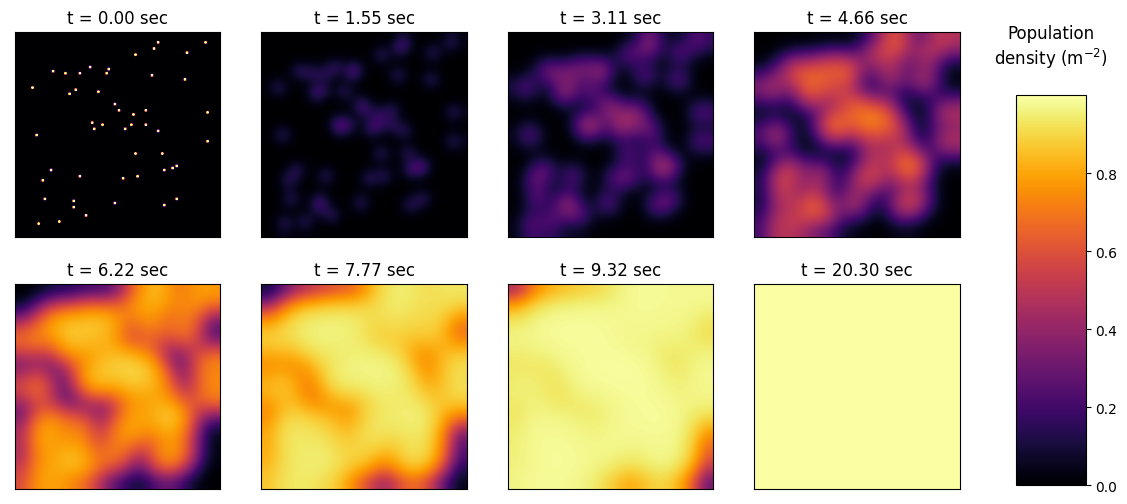
\includegraphics[width=1\linewidth]{Figures/5/5b/neumann_h0.png}
    \caption{Snapshots of the environment at different times with Neumann Boundary Conditions ($r=0.9,h=0$)}
\end{figure}

\begin{figure}[H]
    \centering
    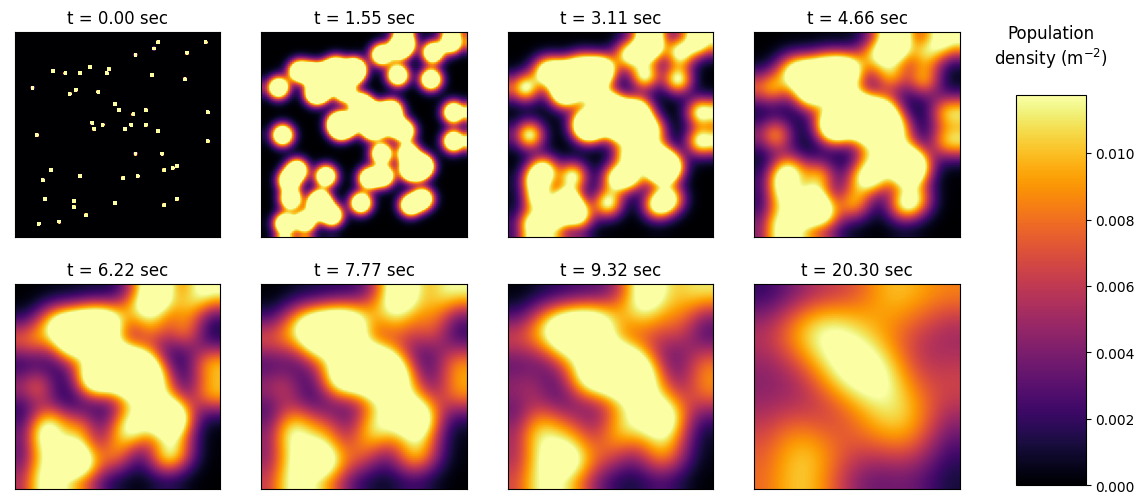
\includegraphics[width=1\linewidth]{Figures/5/5b/neumann_h9.png}
    \caption{Snapshots of the environment at different times with Neumann Boundary Conditions ($r=0.9,h=0.9$)}
\end{figure}

\begin{figure}[H]
    \centering
    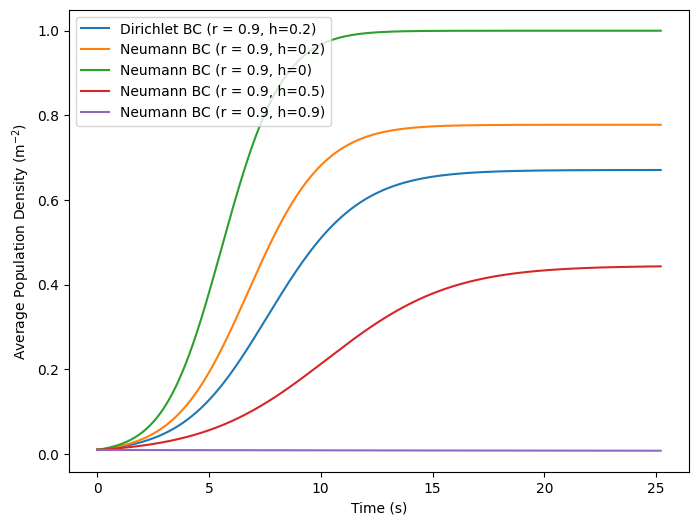
\includegraphics[width=0.6\linewidth]{Figures/5/5b/densities.png}
    \caption{The average population density as a function of time for above-shown simulations.}
\end{figure}

\subsection{Modelling the spread of individuals for a rough terrain}
The third assumption in the previous section assumes a smooth terrain where it is equally easy for individuals to travel in any direction. However, this is rarely the case, as the terrain may have various deformities which affect population diffusion. We will now try to model this mathematically.

For rough terrain, described by a 2D scalar function $T(x, y)$, the actual form of the spatial component of Eq. \ref{diff+h} becomes $\nabla \cdot T(x, y) \nabla u$. Which means,

\begin{align}
    \frac{\partial u}{\partial t} = ru\left(1-\frac{u}{K}\right) - hu + \nabla \cdot (T(x, y) \nabla u)
\end{align}

\subsubsection{Theoretical Approach}
We can choose any $T(x,y)$ that is positive in our domain and perform the operation $\nabla \cdot (T\,\nabla u)$ as,

\begin{align}
    \nabla \cdot (T\,\nabla u) &= \nabla \cdot \left(T\frac{\partial u}{\partial x} \hat{x} + T\frac{\partial u}{\partial y} \hat{y} \right) \nonumber\\
&= \frac{\partial}{\partial x}\left(T\frac{\partial u}{\partial x}\right)  + \frac{\partial}{\partial y}\left(T\frac{\partial u}{\partial y}\right) \nonumber\\
&= \frac{\partial T}{\partial x}\frac{\partial u}{\partial x} + T\frac{\partial^2 u}{\partial x^2} + \frac{\partial T}{\partial y}\frac{\partial u}{\partial y} + T\frac{\partial^2 u}{\partial y^2} \nonumber\\
&= T\,\nabla^2 u + \frac{\partial T}{\partial x}\frac{\partial u}{\partial x} + \frac{\partial T}{\partial y}\frac{\partial u}{\partial y}
\end{align}

Now consider only the $x$ coordinate. We can approximate for a fixed $y$,

\begin{align}
    \frac{\partial T}{\partial x}\frac{\partial u}{\partial x} &\approx \frac{T(x-dx)[u(x-dx)-u(x)] + T(x+dx)[u(x+dx)-u(x)]}{2\,dx^2}\\
T\,\nabla^2 u &\approx \frac{u(x-dx)-2u(x)+u(x+dx)}{2\,dx^2}T(x)
\end{align}

Hence, for a fixed $t$ the full divergence term becomes, 

\begin{align}
\nabla \cdot (T\,\nabla u)|_{(x,y)} = \frac{1}{2\,dx^2} & \Bigl\{ T(x,y) [u(x-dx,y)+u(x+dx,y)+u(x,y-dy)+u(x,y+dy)-4u(x,y)] \Bigl. \nonumber
\\ &+T(x-dx,y)[u(x-dx,y)-u(x,y)] + T(x+dx,y)[u(x+dx,y)-u(x,y)] \nonumber\\ 
&\Bigl. +
T(x,y-dx)[u(x,y-dx)-u(x,y)]+T(x,y+dx)[u(x,y+dx)-u(x,y)]\Bigl\}
\end{align}

Or in terms of coordinates $(i,j)$,

\begin{align}
\nabla \cdot (T\,\nabla u)|_{i,j} = \frac{1}{2\,\Delta x^2} & \Bigl\{ T_{i,j} [u_{i-1,j}+u_{i+1,j}+u_{i,j-1}+u_{i,j+1}-4u_{i,j}] \Bigl. \nonumber
\\ &+T_{i-1,j}[u_{i-1,j}-u_{i,j}] + T_{i+1,j}[u_{i+1,j}-u_{i,j}] \nonumber\\ 
&\Bigl. +
T_{i,j-1}[u_{i,j-1}-u_{i,j}]+T_{i,j+1}[u_{i,j+1}-u_{i,j}]\Bigl\}\\
\text{thus, }u_{i,j}^{(t+1)} &= u_{i,j}^{(t)} + \Delta t\left[(r-h)u_{i,j}^{(t)} - \frac{r(u_{i,j}^{(t)})^2}{K} + \nabla \cdot (T\,\nabla u)|_{i,j}^{(t)}\right]
\end{align}

\subsubsection{Implementation}
We can implement the terrain function in our environment using \verb|np.meshgrid()| function. Here, we have modelled 4 terrains as shown below, but this method will work for any non-negative terrain function $T(x,y)$.

\begin{lstlisting}[language=Python, caption=Code to model the rough terrains]
def gauss2d(x, y, cx=0.5, cy=0.5):
    # gaussian in domain [0,1] x [0,1]
    z = np.exp(-(x-cx)**2-(y-cy)**2)
    return z

def gauss2d_inv(x, y, cx=0.5, cy=0.5):
    # inverted gaussian function
    z = 1-np.exp(-(x-cx)**2-(y-cy)**2)
    return z

def twohills(x, y):
    # a combination of two gaussian hills
    z = 1.04-np.exp((-(x-0.2)**2-(y-0.3)**2)/0.15)-np.exp((-(x-0.8)**2-(y-0.7)**2)/0.1)
    return z

def ridge(x,y):
    # a terrain function that looks like a ridge
    return np.sin((x+3)*(y-0.5)**2)

n = 100
X    = np.linspace(0, 1, n)
Y    = np.linspace(0, 1, n)
X, Y = np.meshgrid(X, Y)

terrain1 = gauss2d(X,Y)
terrain2 = gauss2d_inv(X,Y, cx=0.2, cy=0.4)
terrain3 = twohills(X,Y)
terrain4 = ridge(X,Y)
\end{lstlisting}

\begin{figure}[H]
    \centering
    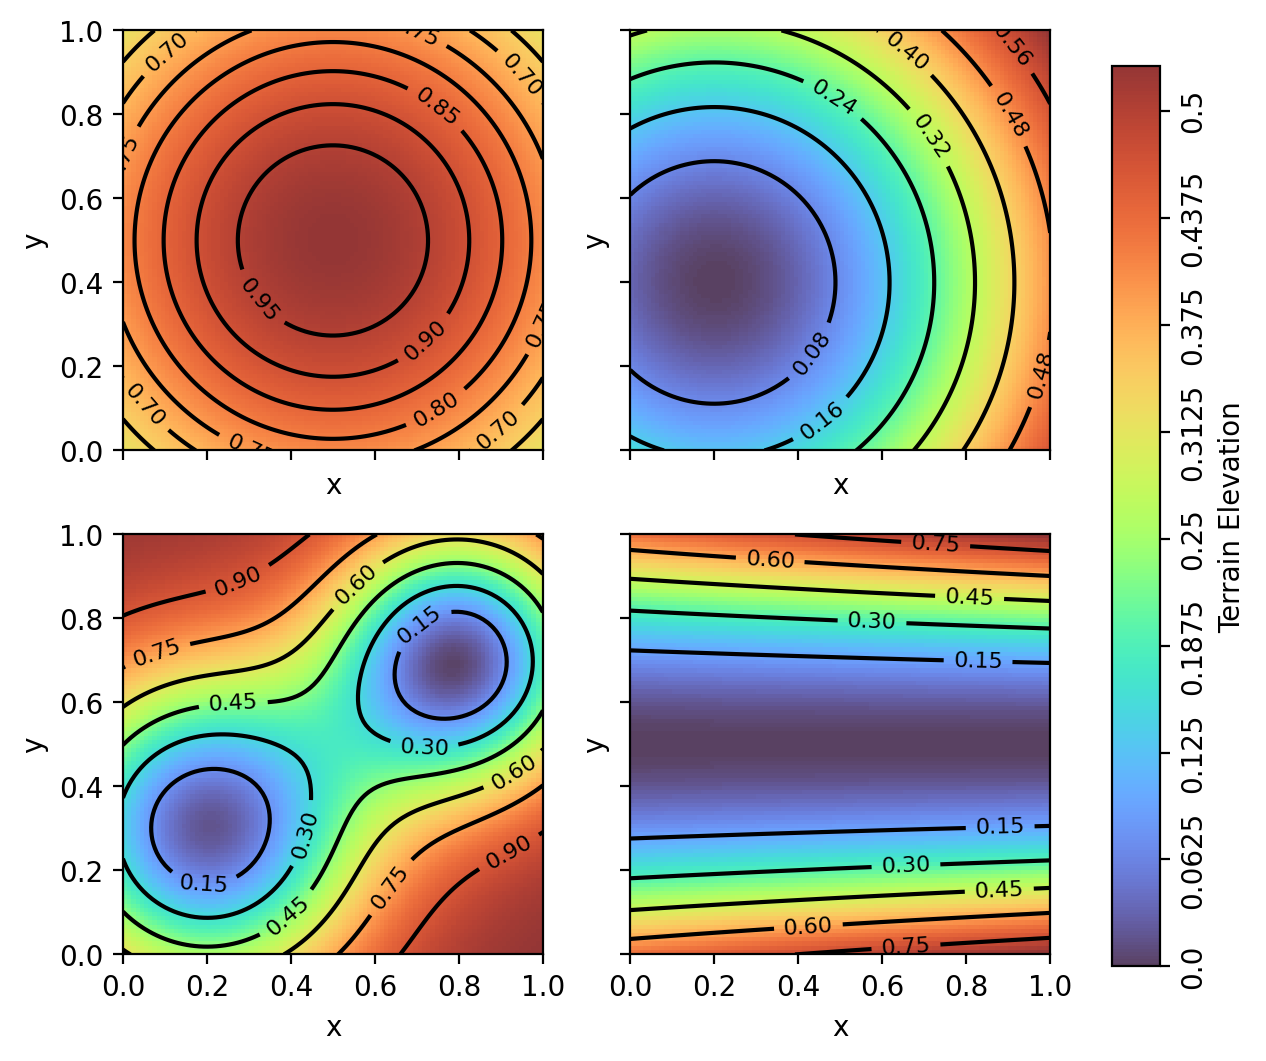
\includegraphics[width=0.7\linewidth]{Figures/5/5c/terrains.png}
    \caption{Contour Plots of the terrains functions we used for the environment}
\end{figure}

The only modification to the \verb|solve_pde()| function defined earlier would be the addition of the divergence term.

\begin{lstlisting}[language=Python, caption=Modified PDE solver function]
@numba.jit("(f8[:,:,:], f8, f8, f8)", nopython=True, nogil=True, fastmath = True)
def solve_pde(environment, K, r, h):
    cs = environment[0].copy() #current state
    length = len(cs[0])
    density = np.zeros(times)
    density[0] = np.average(cs) # average population density
    cf = 0 # current frame
    D = terrain

    for t in range(1, times):
        ns = cs.copy() # new state

        for i in range(1, length-1):
            for j in range(1, length-1):
                growth = dt*((r-h)*cs[j][i] - (r*cs[j][i]**2)/K)
                diffusion = (dt/2*dx**2)* (D[j,i] *(cs[j, i-1]+cs[j, i+1]+cs[j-1,i]\
                                                   +cs[j+1,i]-4*cs[j,i]) +\
                                         D[j-1,i]*(cs[j-1,i]-cs[j,i])+\
                                         D[j+1,i]*(cs[j+1,i]-cs[j,i])+\
                                         D[j,i-1]*(cs[j,i-1]-cs[j,i])+\
                                         D[j,i+1]*(cs[j,i+1]-cs[j,i]))
                ns[j][i] = cs[j][i] + growth + diffusion

        # Implementing Neumann BCs
        ns[:,0] = ns[:,1] # left boundary
        ns[:,-1] = ns[:,-2] # right boundary
        ns[0,:] = ns[1,:] # top boundary
        ns[-1,:] = ns[-2,:] # bottom boundary
        
        density[t] = np.average(cs)
        cs = ns.copy()
        if t%f==0: # take snapshot
            cf = cf + 1
            environment[cf] = cs
            
    return environment, density
\end{lstlisting}

\subsubsection{Results} \label{rough_section}

Here again, the population diffuses slowly until it reaches saturation. However, this time, the diffusion is not uniform and is dependent on the terrain function.

\begin{figure}[H]
    \centering
    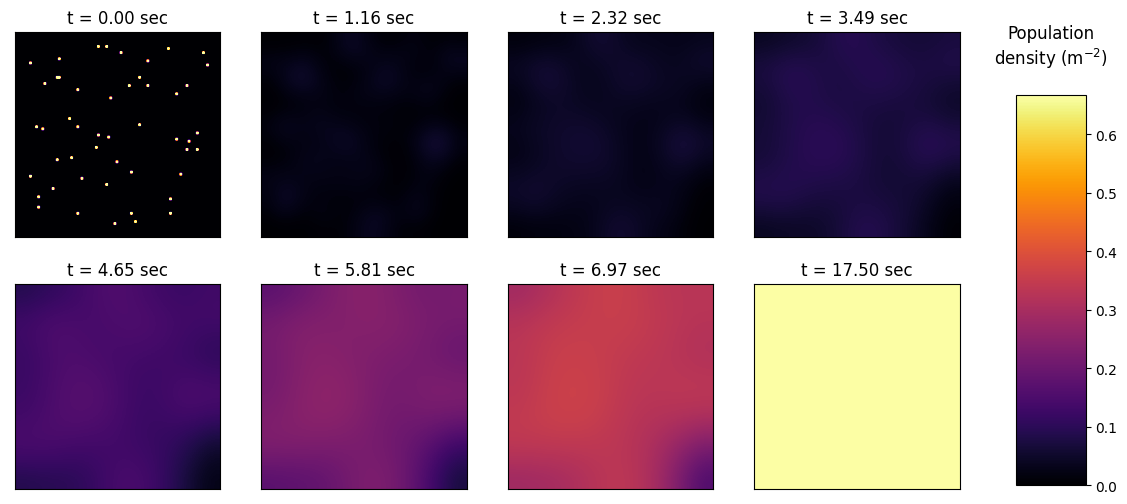
\includegraphics[width=1\linewidth]{Figures/5/5c/terrain1_spread.png}
    \caption{Snapshots of the environment at different times with a Gaussian Terrain ($r=0.9,h=0.2$)}
\end{figure}

\begin{figure}[H]
    \centering
    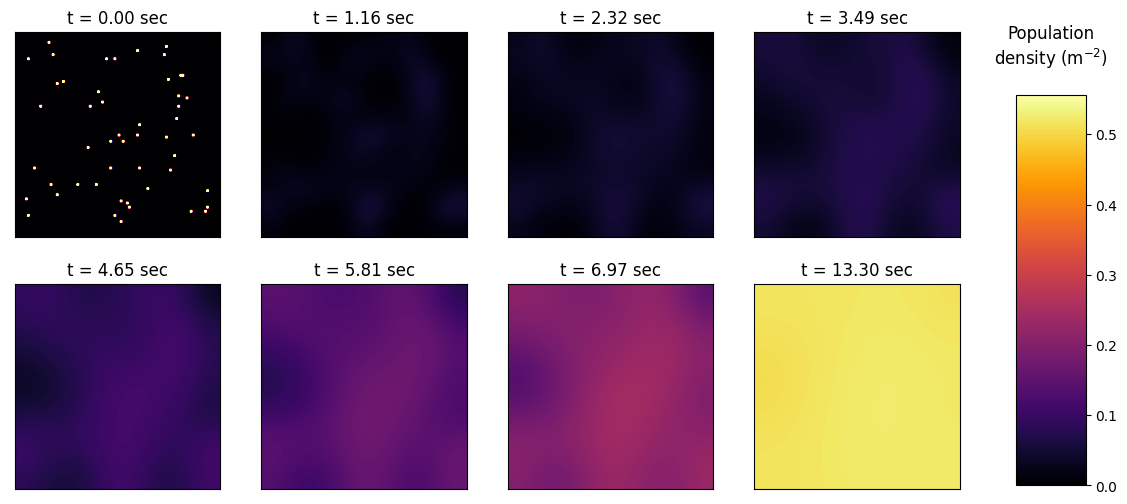
\includegraphics[width=1\linewidth]{Figures/5/5c/rough_gauss_r4.png}
    \caption{Snapshots of the environment at different times with a Gaussian Terrain ($r=0.9,h=0.4$). Here while the simulation looks similar to the one above the final saturated value is lesser due to the higher hunting rate.}
\end{figure}

\begin{figure}[H]
    \centering
    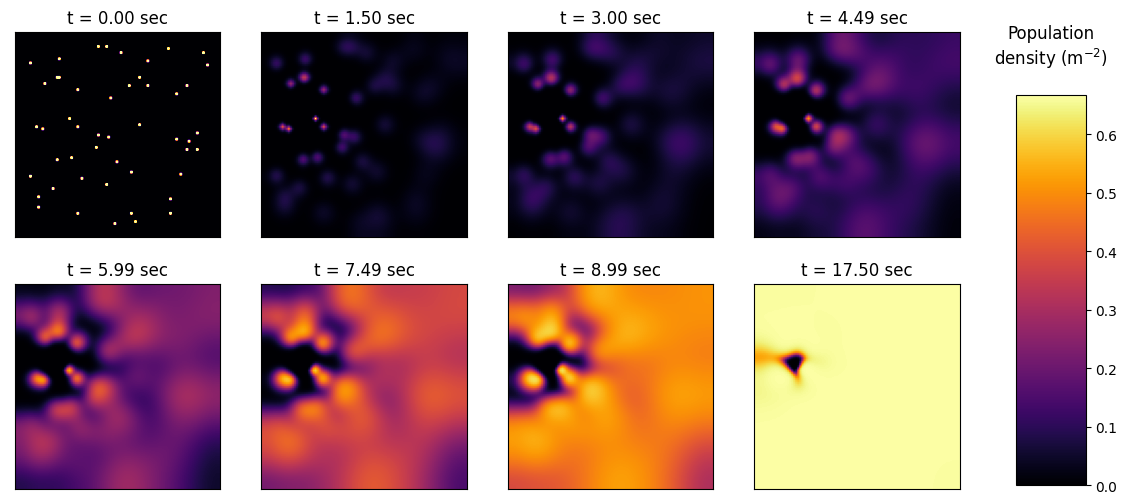
\includegraphics[width=1\linewidth]{Figures/5/5c/terrain2_spread.png}
    \caption{Snapshots of the environment at different times with an inverted Gaussian Terrain ($r=0.9,h=0.2$)}
\end{figure}

\begin{figure}[H]
    \centering
    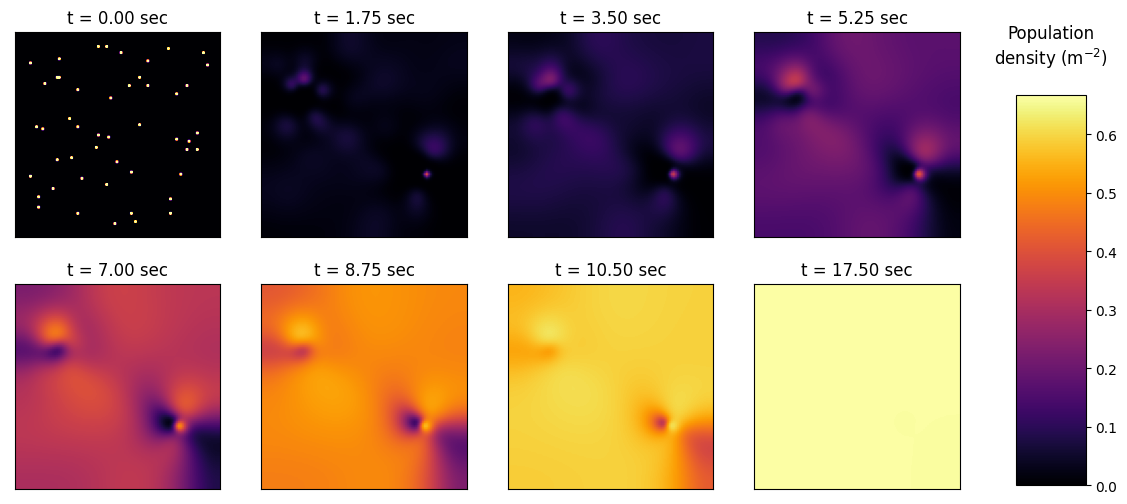
\includegraphics[width=1\linewidth]{Figures/5/5c/terrain3_spread.png}
    \caption{Snapshots of the environment at different times with a Gaussian Terrain with two peaks ($r=0.9,h=0.2$)}
\end{figure}

\begin{figure}[H]
    \centering
    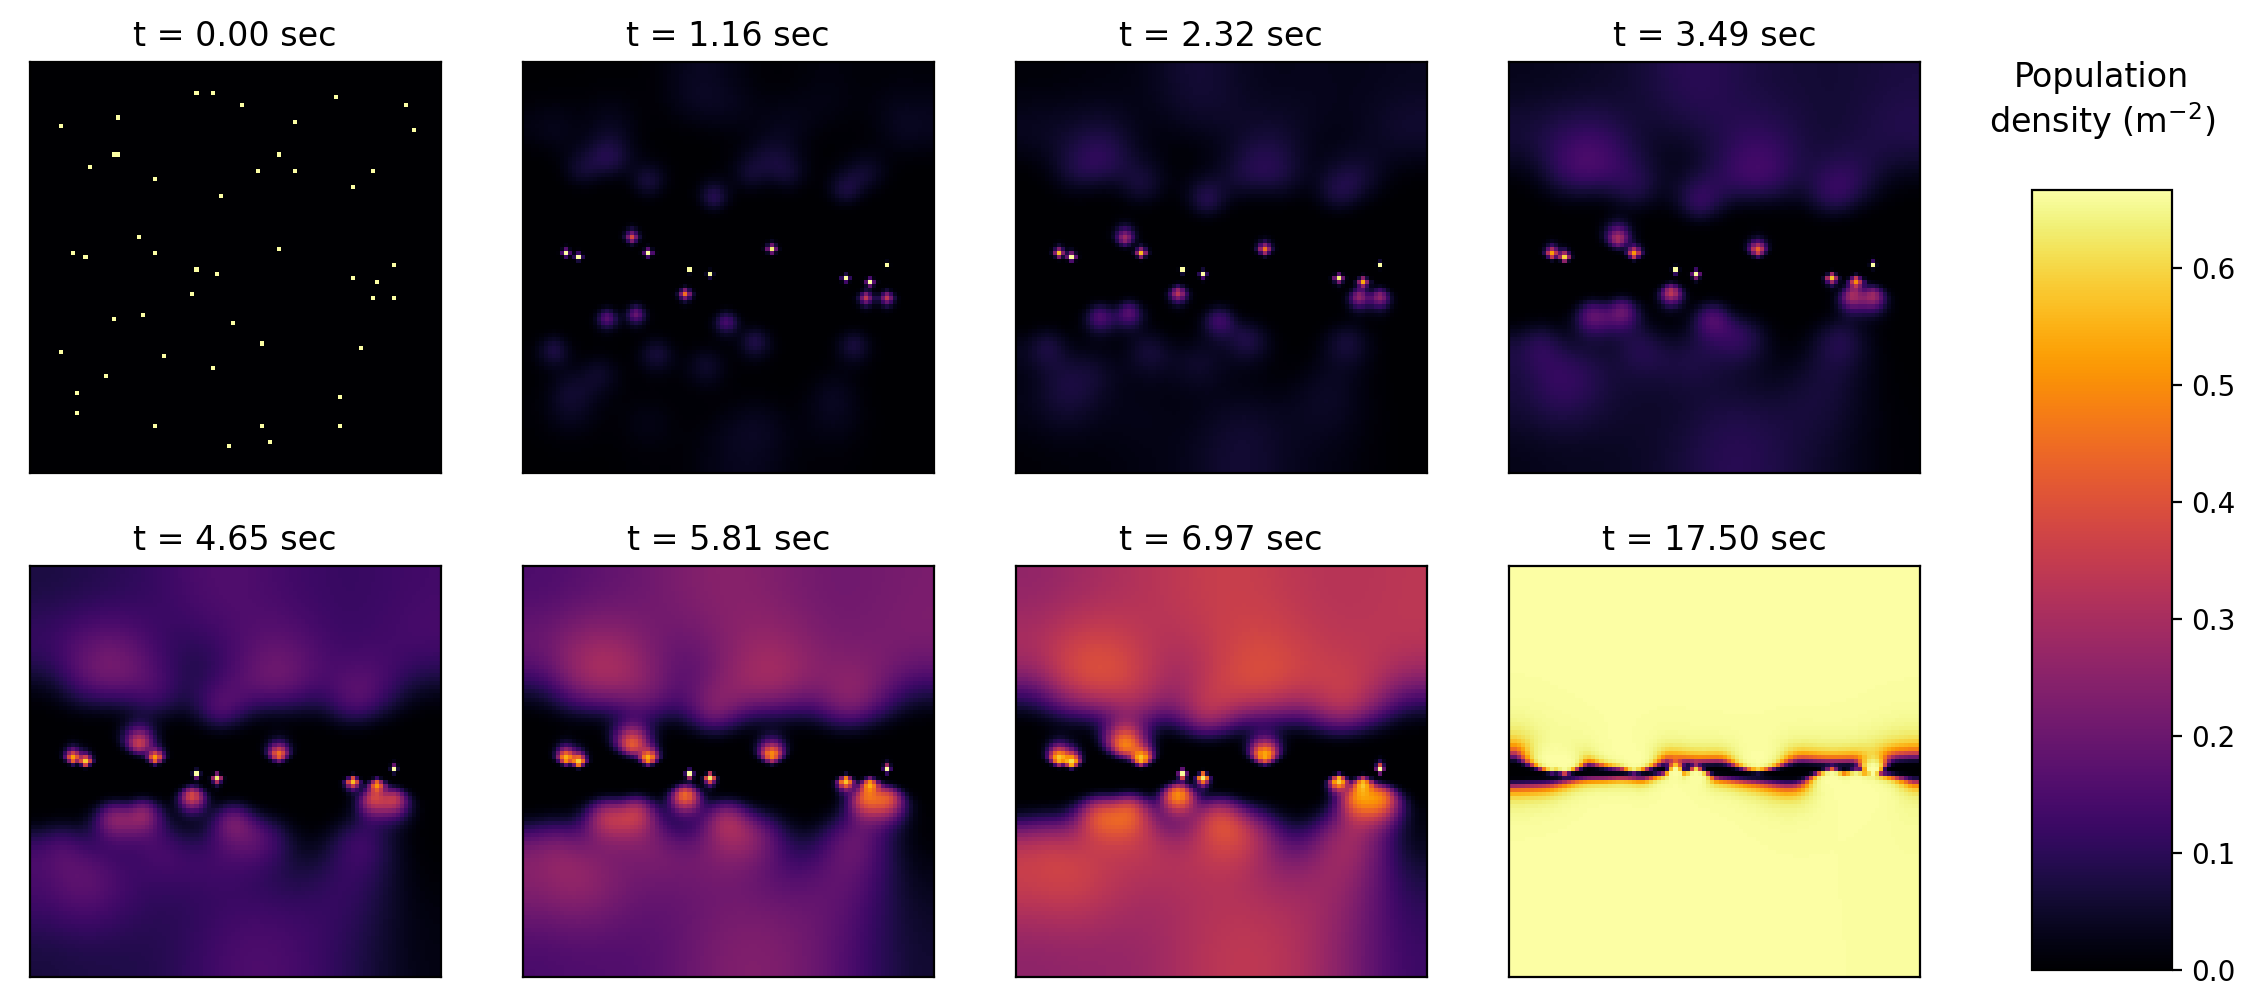
\includegraphics[width=1\linewidth]{Figures/5/5c/terrain4_spread.png}
    \caption{Snapshots of the environment at different times with the ridge-like terrain ($r=0.9,h=0.2$)}
\end{figure}


\begin{figure}[H]
    \centering
    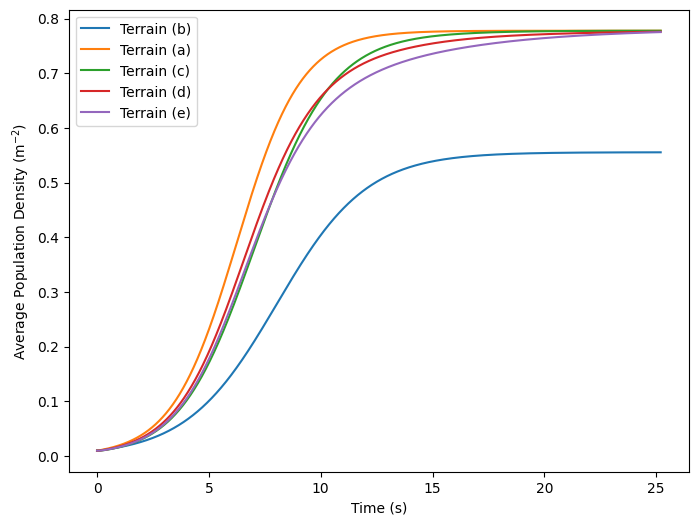
\includegraphics[width=0.5\linewidth]{Figures/5/5c/densities.png}
    \caption{The average population density as a function of time for above-shown simulations in order. As you can see, all environments evetually saturate to the same value, except for the one with a lower $K$ value.}
\end{figure}

% \subsection{Discussion}

The simulations videos for most of the simulations in Section \ref{rough_section} are available \href{https://gayatri-p.github.io/p346-computational-physics/hunting3.html#simulation-for-each-terrain}{here}.

